%%%%%%%%%%%%%%%%%%%%%%%%%%%%%%%%%%%%%%%%%%%%%%%%%%%%%%%%%%%%%%%%%%%%%%%%%%%%%%%%%%%%%%%%%%%%%%
%%%%%%%%%%%%%%%%%%%%%%%%%%%%%%%%%%%%%%%%%%%%%%%%%%%%%%%%%%%%%%%%%%%%%%%%%%%%%%%%%%%%%%%%%%%%%%
%%%%%%%%%%% systemOverview
%%%%%%%%%%%%%%%%%%%%%%%%%%%%%%%%%%%%%%%%%%%%%%%%%%%%%%%%%%%%%%%%%%%%%%%%%%%%%%%%%%%%%%%%%%%%%%
%%%%%%%%%%%%%%%%%%%%%%%%%%%%%%%%%%%%%%%%%%%%%%%%%%%%%%%%%%%%%%%%%%%%%%%%%%%%%%%%%%%%%%%%%%%%%%


% \cleardoublepage
\chapter{System Overview}
\label{sec:systemOverview}

\section{Overview}
This chapter gives a high lever overview of the the algorithms implemented into the GPU.
A block diagram is shown in Figure \ref{fig:simpleBlockDiagram}.
The algorithms implemented in GPUs will briefly be explained.
Chapter \ref{sec:eq_eq} explains the computation and application of the equalizers at a lower level.
A simple block Diagram is shown in Figure \ref{fig:simpleBlockDiagram}.

This chapter will proceed as follows, 
section \ref{sec:preamble_detection} will explain the algorithm used to find the preambles and packetize the received signal,
section \ref{sec:frequency_offset_estimation_and_compensation} will explain the frequency offset estimator and frequency offset compensation,
section \ref{sec:channel_estimation} will explain channel channel estimation,
section \ref{sec:noise_variance_estimation} will explain noise variance,
section \ref{sec:oqpsk_detector} will explain the GPU implementation of the OQPSK detector.
The explanation of the GPU implantation of the equalizers will be explained in much detail in Chapter \ref{sec:eq_eq}.
\begin{figure}
	\centering\includegraphics[width=6in]{figures/systemOverview/blockDiagram.pdf}
	\caption{This a simple block diagram of what the GPU does.}
	\label{fig:simpleBlockDiagram}
\end{figure}



















\subsection{Preamble Detection}
\label{sec:preamble_detection}
The received samples in this project has the iNET packet structure shown in Figure \ref{fig:packet}.
The iNET packet consists of a preamble and ASM periodically inserted into the data stream.
The iNET preamble and ASM bits are inserted every 6144 data bits.
The received signal is sampled at 2 samples/bit, making a iNET packet $\Lpkt$ long or $12672$ samples.
The iNET preamble comprises eight repetitions of the 16-bit sequence $\text{CD98}_\text{hex}$ and the ASM field
\begin{equation}
034776C72728950B0_\text{hex}
\end{equation}
\begin{figure}
	\centering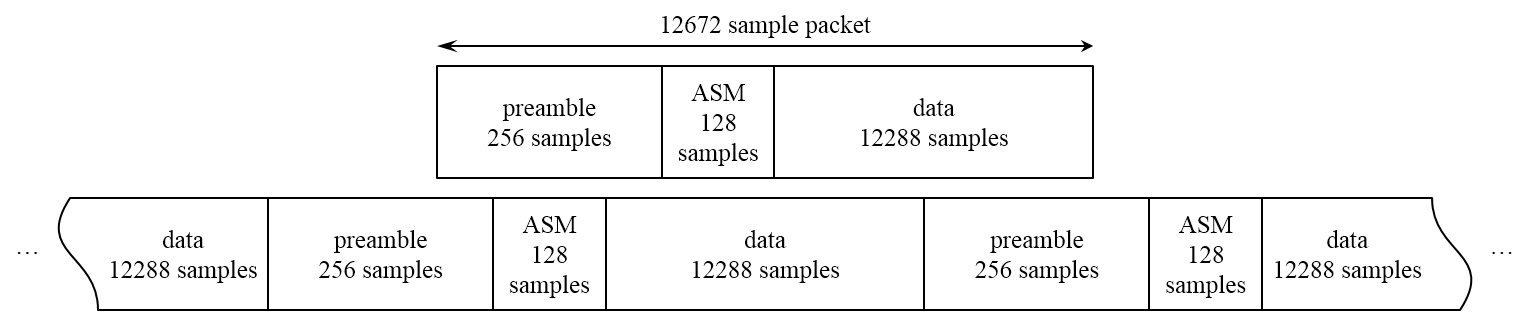
\includegraphics[width=\textwidth/10*11]{figures/gpu/packet.png}
	\caption{The iNET packet structure.}
	\label{fig:packet}
\end{figure}

To compute data-aided preamble assisted equalizers, preambles in the received signal are found then used to estimate various parameters.
The goal of the preamble detection step is to "packetize" the received samples into vectors with the packet structure shown in Figure \ref{fig:packet}. Each packet of received samples contains a $\Lp$ preamble samples, $\Lasm$ ASM samples and $\Lasm$ data samples.

Before the received samples can be packetized, the preambles are found using a preamble detector explained in \cite{preamble_detector}.
The preamble detector output $L(u)$ is computed by 
\begin{equation}
	L(u) = \sum_{m=0}^{7}
		\left[ I^2(n,m) + Q^2(n,m) \right]
	\label{eq:gpu-L-4}
\end{equation}
where the inner summations are
\begin{multline}
	I(n,m) \approx \sum_{\ell\in\mathcal{L}_1}r_R(\ell+32m+n)
			- \sum_{\ell\in\mathcal{L}_2}r_R(\ell+32m+n)
			+ \sum_{\ell\in\mathcal{L}_3}r_I(\ell+32m+n)
			- \sum_{\ell\in\mathcal{L}_4}r_I(\ell+32m+n)
			\\
			+ 0.7071 \left[
				\sum_{\ell\in\mathcal{L}_5}r_R(\ell+32m+n)
				- \sum_{\ell\in\mathcal{L}_6}r_R(\ell+32m+n)
			\right. \\
			\left.
				+ \sum_{\ell\in\mathcal{L}_7}r_I(\ell+32m+n)
				- \sum_{\ell\in\mathcal{L}_8}r_I(\ell+32m+n)
			\right],
	\label{eq:gpu-L-pedone-geoghegan-2}
\end{multline}
and
\begin{multline}
	Q(n,m) \approx \sum_{\ell\in\mathcal{L}_1}r_I(\ell+32m+n)
			- \sum_{\ell\in\mathcal{L}_2}r_I(\ell+32m+n)
			\\
			- \sum_{\ell\in\mathcal{L}_3}r_R(\ell+32m+n)
			+ \sum_{\ell\in\mathcal{L}_4}r_R(\ell+32m+n)
			\\
			+ 0.7071 \left[
				\sum_{\ell\in\mathcal{L}_5}r_I(\ell+32m+n)
				- \sum_{\ell\in\mathcal{L}_6}r_I(\ell+32m+n)
			\right. \\
			\left.
				- \sum_{\ell\in\mathcal{L}_7}r_R(\ell+32m+n)
				+ \sum_{\ell\in\mathcal{L}_8}r_R(\ell+32m+n)
			\right]
		\label{eq:gpu-L-pedone-geoghegan-3}
\end{multline}
with
\begin{equation}
	\begin{split}
	\mathcal{L}_1 &= \{ 0, 8, 16, 24 \}\\
	\mathcal{L}_2 &= \{ 4, 20 \}\\
	\mathcal{L}_3 &= \{ 2, 10, 14, 22 \}\\
	\mathcal{L}_4 &= \{ 6, 18, 26, 30 \}\\
	\mathcal{L}_5 &= \{ 1, 7,  9, 15, 17, 23, 25, 31 \}\\
	\mathcal{L}_6 &= \{ 3, 5, 11, 12, 13, 19, 21, 27, 28, 29 \}\\
	\mathcal{L}_7 &= \{ 1, 3,  9, 11, 12, 13, 15, 21, 23 \}\\
	\mathcal{L}_8 &= \{ 5, 7, 17, 19, 25, 27, 28, 29, 31 \}.
\end{split}
\label{eq:gpu-L-pedone-geoghegan-4}
\end{equation}
Figure \ref{fig:L_2_packets} shows $2\Lpkt$ samples of the preamble detector output $L(u)$.
\begin{figure}
	\centering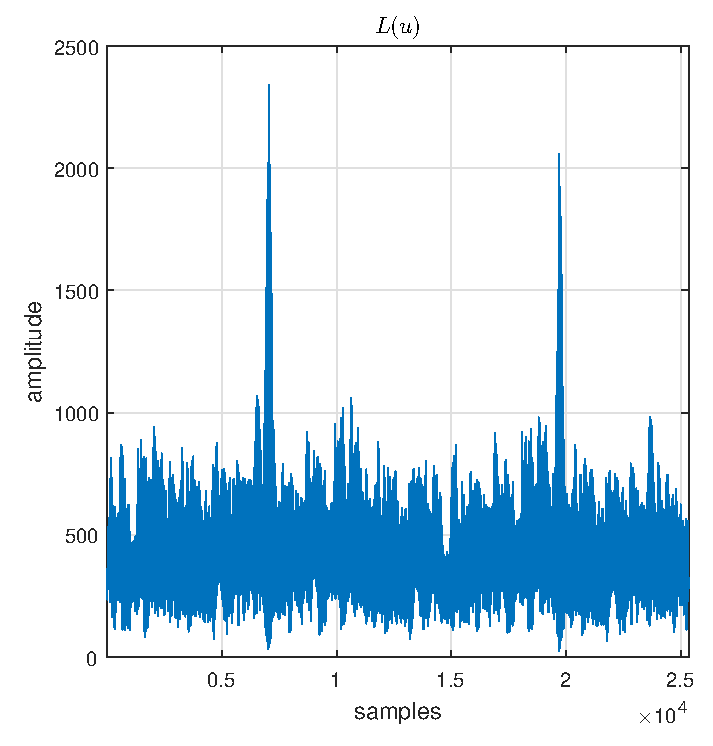
\includegraphics[width=5in]{figures/gpu/L_2_packets.eps}
	\caption{The output of the Preamble Detector $L(u)$.}
	\label{fig:L_2_packets}
\end{figure}
The start of a preamble is indicated by a local maximum of the preamble detector output.
Using the index of the local maximums, the received samples are packetized.
The vector $\rpkt$ as shown in Figure \ref{fig:simpleBlockDiagram} contains $12672$ samples of data with the packet structure shown in Figure \ref{fig:packet}.

The preamble detection algoritm in Equations \eqref{eq:gpu-L-4}-\eqref{eq:gpu-L-pedone-geoghegan-4} and the local maximum search algorithms are easily implemented into GPUs.
The GPU implementation of these algorithms wont be explained here.

%To find the preambles in the batch, the preamble detector computes the sample correlation function between the received samples and a stored local copy of the known samples of the iNET preamble. 
%The correlation function output is searched for local maximums. 
%In ideal conditions, the local maximums are seperated by $\Lpkt$ samples.
%
%The preamble detector detailed in \cite{preamble_detector} is a highly optimized correlator used to compute to how a signal correlates with the iNET preamble eight repetitions of the 16-bit sequence $\text{CD98}_\text{hex}$.
%%The preamble detector outer summation is
%
%Equations \eqref{eq:gpu-L-4}-\eqref{eq:gpu-L-pedone-geoghegan-4} produce the preamble detector output $L(u)$.
%The equations are easily implemented into GPUs in two steps.
%First launching one thread to compute the inner sums $I(n,m)$ and $Q(n,m)$ for each received sample.
%Second, with the inner sums computed, one thread is launched to compute the outer sum $L(u)$ for each received sample.
%Figure \ref{fig:L_2_packets} shows $2\Lpkt$ samples of the preamble detector output $L(u)$.
%\begin{figure}
%	\centering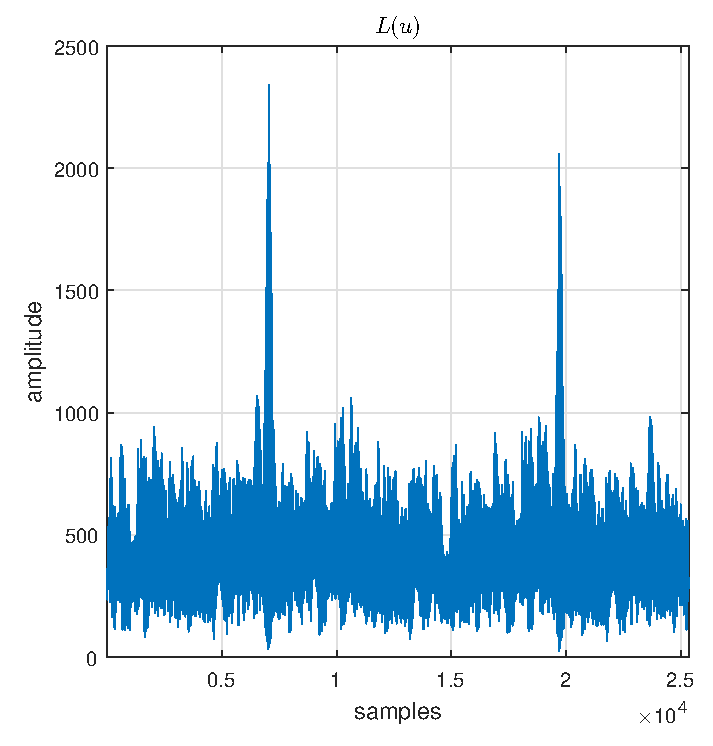
\includegraphics[width=5in]{figures/gpu/L_2_packets.eps}
%	\caption{The output of the Preamble Detector $L(u)$.}
%	\label{fig:L_2_packets}
%\end{figure}
%
%\subsubsection{Searching for the Starting Indices}
%Equipped with the preamble detector output, $L(u)$ is searched for local maximums or peaks to find the starting index for each preamble.
%The first maximum or peak in Figure \ref{fig:L_2_packets} shows the first packet starts at sample index $7040$ and the second at $19712$.
%The difference between these sample indices is $\Lpkt$, this difference agrees with the packet length shown in Figure \ref{fig:packet}.
%
%With ideal received samples, 512 samples of $L(u)$ looks like Figure \ref{fig:L_corr_creepy}(a).
%The structure of the correlation peaks still occur when the signal to noise ratio is low, as shown in Figure \ref{fig:L_corr_creepy}(b).
%But when the signal to noise ratio is low and major multipath distortion happen, the correlation peaks look like Figures \ref{fig:L_corr_creepy}(c) and (d).
%
%The preamble detector output $L(u)$ has unique properties because the 16-bit sequence $\text{CD98}_\text{hex}$ sampled at 2 samples/bit.
%A local maximum occurs when $u$ is the starting index of a preamble. 
%Side peaks occur because the samples of the preamble are highly correlated when offset by 32 samples.
%The preamble detector output has seven side peaks separated by 32 samples because the repeated 32 sample pattern.
%The Figures in \ref{fig:L_corr_creepy} show $L(u)$ around correlation peaks.
%
%The preamble detector output is searched for local maximums separated by $\Lpkt$.
%To ensure only one set of correlation peaks is searched for a local maximum, $\Lpkt$ samples are searched using windows that are centered on one correlation peak set.
%
%If the search windows aren't centered on the correlation peaks, the $\Lpkt$ samples searched could find an adjacent side peak rather than the desired local maximum.
%The side peaks in Figure \ref{fig:L_corr_creepy}(a) are much larger than the main correlation peaks in Figures \ref{fig:L_corr_creepy}(c) or (d).
%\begin{figure}
%	\begin{center}
%		\begin{tabular}{cc}
%			\begin{minipage}[c]{3in}
%				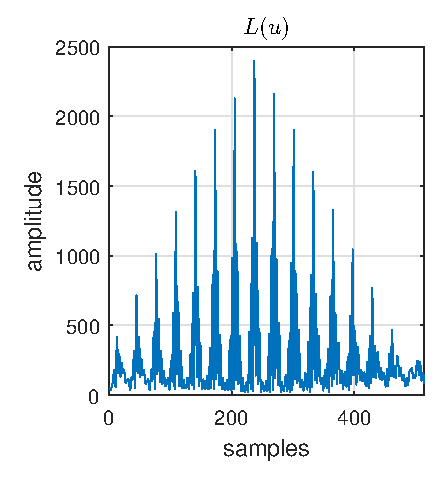
\includegraphics[width=3in]{figures/gpu/L_corr_8_clean.eps}
%			\end{minipage} 
%			&  
%			\begin{minipage}[c]{3in}
%				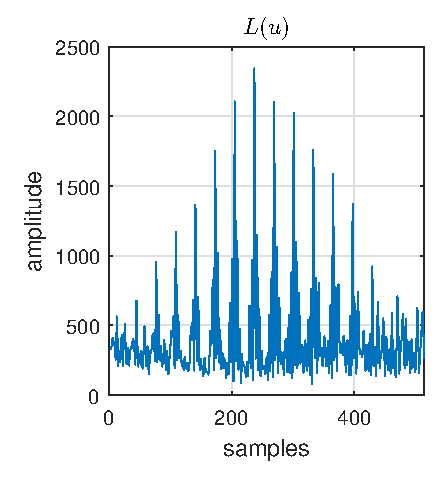
\includegraphics[width=3in]{figures/gpu/L_corr_8_noise.eps}
%			\end{minipage} \\[12pt]
%			
%			\quad\quad\quad\quad(a)
%			&
%			\quad\quad\quad\quad(b) \\[12pt]
%			
%			\begin{minipage}[c]{3in}
%				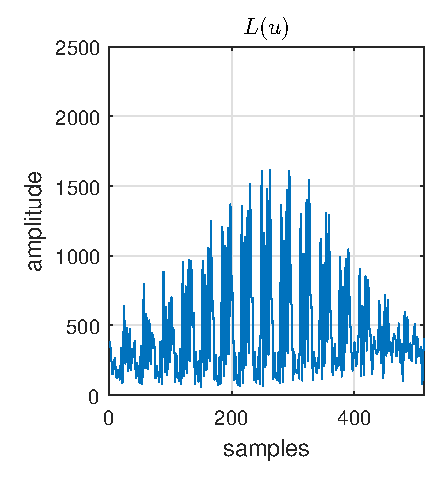
\includegraphics[width=3in]{figures/gpu/L_corr_17_creepy.eps}
%			\end{minipage} 
%			&  
%			\begin{minipage}[c]{3in}
%				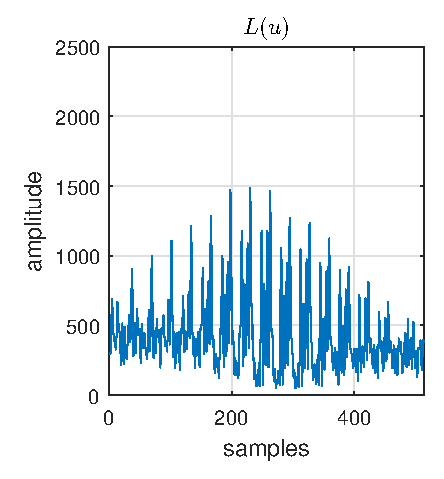
\includegraphics[width=3in]{figures/gpu/L_corr_18_creepy.eps}
%			\end{minipage} \\[12pt]
%			
%			\quad\quad\quad\quad(c)
%			&
%			\quad\quad\quad\quad(d)
%			
%		\end{tabular}
%	\end{center}
%	\caption{Detailed view of $L(u)$. 
%			(a): correlation peaks of a distortion free and noiseless signal; 
%			(b): correlation peaks of a distortion free but noisy signal with $E_b/N_0 = 0$dB; 
%			(c): correlation peaks of a distorted and noisy signal with $E_b/N_0 = 0$dB;
%			(d): correlation peaks of a distorted and noisy signal with $E_b/N_0 = 0$dB}
%	\label{fig:L_corr_creepy}
%\end{figure}
%
%To center the search windows, an initial search is done on the first $2\Lpkt$ $L(u)$ samples to estimate the index of the first preamble $\hat{i}_0$.
%Figure \ref{fig:L_windows} shows an example of safe search windows centered on expected preamble starting locations.
%One GPU thread per search window is launched to parallelize the search.
%\begin{figure}
%	\centering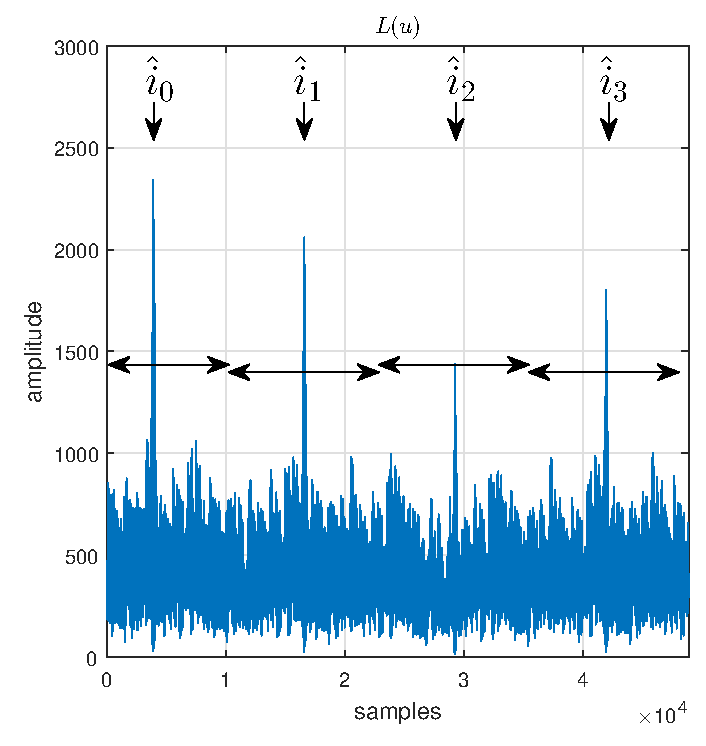
\includegraphics[width=5in]{figures/gpu/L_windows.eps}
%	\caption{Safe search windows defined to search only one preamble correlation peak.}
%	\label{fig:L_windows}
%\end{figure}
%The vector
%\begin{align}
%\hat{\mathbf{i}}
%=     
%\begin{bmatrix}
%\hat{i}_0 	\\
%\hat{i}_1	\\
%\vdots		\\
%\hat{i}_{3103}	\\
%\hat{i}_{3104}  		
%\end{bmatrix}
%\label{eq:preamble_det_i_hat}
%\end{align}
%is built by the GPU window search kernel.
%The vector $\hat{\mathbf{i}}$ is a vector of rough estimates of where the preambles should be located.
%The windows in the GPU search kernel are centered on elements of $\hat{\mathbf{i}}$ as shown in Figure \ref{fig:L_windows}.
%Adjustments are made to the peak index vector $\hat{\mathbf{i}}$ is checked for $\Lpkt$ spacing.
%
%\clearpage
%\subsubsection{Packetizing the Samples}
%Finally, with the best estimate of the preamble starting locations, the received samples can be packetized.
%Using $\hat{\mathbf{i}}$, the GPU launches one thread per received sample to packetize $r(n)$ into $\mathbf{r}_\text{pkt}$ as shown in Figure \ref{fig:packetized}. 
%The structure of $\mathbf{r}_\text{pkt}$ majorly simplifies indexing and removes the need for $\hat{\mathbf{i}}$.
%\begin{equation}
%\mathbf{r}_\text{pkt} = 
%\begin{bmatrix}
%r(\hat{i}_0) 			\\
%r(\hat{i}_0+1) 		\\
%\vdots			\\
%r(\hat{i}_0+12670)\\
%r(\hat{i}_0+12671)\\
%r(\hat{i}_1) 			\\
%r(\hat{i}_1+1) 		\\
%\vdots			\\
%r(\hat{i}_{3103}+12670)\\
%r(\hat{i}_{3103}+12671)\\
%\end{bmatrix}
%\end{equation}
%\begin{figure}
%	\centering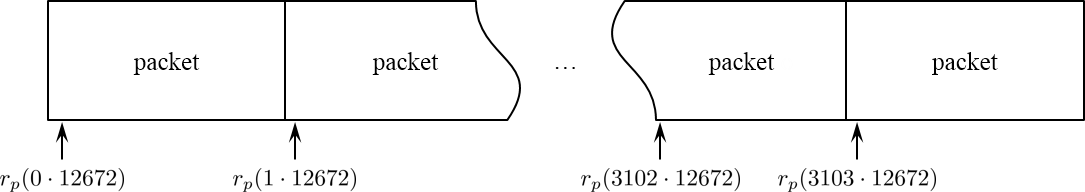
\includegraphics[width=\textwidth/10*9]{figures/gpu/packetized.png}
%	\caption{The packetized structure of the received signals after the frame synchronization step.}
%	\label{fig:packetized}
%\end{figure}

%\subsection{Frequency Offset Estimation and Compensation}
%\label{sec:frequency_offset_estimation_and_compensation}
%With the vector $\mathbf{r}_\text{pkt}$ built, estimators can now easily use the preamble to estimate various parameters.

\subsubsection{Frequency Offset Compensation}
\label{sec:jeffs_frequencyoffsetestimator}
The frequency offset estimator shown in Figure \ref{fig:simpleBlockDiagram} is an algorithm taken from blah.
With the notation adjusted slightly, the frequency offset estimate is
\begin{equation}
	\hat{\omega}_0 = \frac{1}{L_q} \arg\left\{ \sum_{n=i+2L_q}^{i+7L_q-1} r(n)r^\ast(n-L_q)\right\}
	\label{eq:jeff-ML-w-final3}
\end{equation}
where a frequency offset estimate is produced for every packet in $\rpkt$.

The frequency offset is compensated for by derotating the packetized samples
\begin{equation}
	r(n) = r_\text{pkt} e^{-j\hat{\omega}_0}
	\label{eq:frequency_compensation}
\end{equation}
Equation \eqref{eq:jeff-ML-w-final3} is easily implemented into GPUs. 

\subsection{Channel Estimation}
\label{sec:channel_estimation}

\subsection{Noise Variance Estimation}
\label{sec:noise_variance_estimation}

\subsection{OQPSK Detector}
\label{sec:oqpsk_detector}

%\section{System Pictures}
%
%\section{Block Diagram}
%
%\section{Equations}
%
%\subsection{Estimators}
%\subsubsection{Preamble Detector}
%
%\subsection{Equalizers}
%
%\subsection{Decisions}
